\chapter*{{\normalfont Chapter 3} \\ Localized Solutions of Gross-Pitaevskii Equation with Periodic Pseudopotential}
\addcontentsline{toc}{chapter}{Chapter 3 \quad Localized Solutions of Gross-Pitaevskii Equation with Periodic Pseudopotential}
\label{chapter:III}

\section*{3.1 Objectives}
\addcontentsline{toc}{section}{3.1 \quad Objectives}

In this chapter we apply the coding approach to the Gross-Pitaevskii equation of the form
\begin{equation}
	i \Psi_t + \Psi_{xx} - U(x) \Psi + P(x) |\Psi|^2 \Psi = 0.
\label{eq:gpe}
\end{equation}
Here both potential $U(x)$ and pseudopotential $P(x)$ are periodic functions.
Such equation occurs in physics of Bose-Einstein condensate (BEC) where periodical pseudopotential is achieved by means of the Feshbach resonance controlled by magnetic or optical fields \cite{PollackDriesJunkerChenCorcovilosHulet, ChinGrimmJulienneTsienga, BauerLetterVoRempeDurr}.
Experimentally, the possibility of the periodic modulation of the nonlinearity was demonstrated in \cite{YamazakiTaieSugawaTakahashi}.
One can also find equation \eqref{eq:gpe} in optics where spatial modulation of the Kerr coefficient can be achieved by means of inhomogeneous density of resonant nonlinearity-enhancing dopants implanted into the waveguide \cite{HukriedeRundeKip}.

We are interested in stationary localized solutions of equation \eqref{eq:gpe}, also called as solitons in physical applications.
Strictly speaking, the objects that we are going to study are not solitons in the mathematically rigorous meaning, but rather ``solitary waves'', as they appear in a nonintegrable model.
Nevertheless, the application of the word ``soliton'' to localized pulses in BECs is commonly adopted in physics literature, therefore we also use this word.
Stationary solutions satisfy the ansatz $\Psi(t, x) = u(x) e^{i \omega t}$, where function $u(x)$ is a solution of equation
\begin{equation}
	u_{xx} + Q(x) u + P(x) u^3 = 0, \quad Q(x) = -\omega - U(x).
\end{equation}
Localized solutions satisfy the localization condition
\begin{equation}
	\lim \limits_{x \to \pm \infty} u(x) = 0,
\label{eq:localization}
\end{equation}
which implies that the function $u(x)$ is real, see \cite{AlfimovKonotopSalerno}.
In what follows below we also assume that the potential $U(x)$ is absent, i.e. $U(x) \equiv 0$, so the effects produced by the periodic modulation of the nonlinearity are not obscured by the linear-lattice potential.
Prototypical example of periodic pseudopotential is provided by a function
\begin{equation}
	P(x) = \alpha + \cos 2x, \quad \alpha \in \mathbb{R}.
\label{eq:cosine-pseudopotential}
\end{equation}
Resulting GPE equation takes form
\begin{equation}
	i \Psi_t + \Psi_{xx} + (\alpha + \cos 2x) |\Psi|^2 \Psi = 0,
\label{eq:gpe-cosine}
\end{equation}
where the period of pseudopotential function $P(x)$ is scaled to be $L = \pi$.
Corresponding stationary state equation is
\begin{equation}
	u_{xx} - \omega u + (\alpha + \cos 2x) u^3 = 0.
\label{eq:stationary-cosine}
\end{equation}
Equation \eqref{eq:gpe-cosine} and \eqref{eq:stationary-cosine} are the objects of our analysis during this chapter.
The same model has been previously discussed in literature, see paper \cite{SakaguchiMalomed}.
In \cite{SakaguchiMalomed} only single-peak localized solution, called {\it fundamental soliton} (FS), was studied in details.
For that purpose authors used variational approximation method which requires initial guess of the solution shape.
Such limitation does not allow to find more sophisticated localized solutions.
By using of our coding technique we are going to reveal significantly wider class of stationary localized solutions of Eq.~\eqref{eq:gpe-cosine}.

\section*{3.2 Coding of Solutions}
\addcontentsline{toc}{section}{3.2 \quad Coding of Solutions}

Our approach requires the presence of singular solutions families.
That's why according to Proposition~\ref{prop:singular-families} we assume that $\alpha \in (-1; 1)$, so that function $P(x)$ alternates its sing along the value $x$.
We also assume that $\omega > 0$.
This restriction comes from the obvious condition of the soliton localization, given by Eq.\eqref{eq:localization}.

Let's introduce a Poincar\'e map $\mathcal{P}: \mathbb{R}^2 \to \mathbb{R}^2$ associate with equation \eqref{eq:stationary-cosine} in the same way we did it before in \eqref{eq:poincare-map} assuming $L = \pi$.
Poincar\'e map $\mathcal{P}$ and its inverse $\mathcal{P}^{-1}$ is not defined in the whole plane $(u, u')$ of initial conditions.
We can construct their domains using the scanning technique introduced in Chapter~2. % \ref{chapter:II}
Sets $\mathscr{U}_{\pi}^+$ and $\mathscr{U}_{\pi}^-$ for different parameters $(\omega, \alpha)$ are presented in Figure~\ref{fig:island-set-emergence-cosine}.
Numerical results allows us to conclude that the sets $\mathscr{U}_{\pi}^{\pm}$ are unbounded spirals with infinite number of rotations around the origin, similar to what we saw previously for equation \eqref{eq:stationary-piecewise}.
According to the Proposition~\ref{prop:domain-reflection} these sets are related with a reflection with respect to the $u'$ axis, i.e. $\mathscr{U}_{\pi}^- = I \mathscr{U}_{\pi}^+$.
Their thicknesses depend on the parameter $\alpha$.
If these sets are thin enough their intersection $\mathscr{U}_{\pi} = \mathscr{U}_{\pi}^+ \cap \mathscr{U}_{\pi}^-$ form an island set.
In Figure~\ref{fig:island-set-emergence-cosine} panels (a), (b), and (c) resulting set $\mathscr{U}_{\pi}$ cannot be regarded as island set.
In panel (d) $\mathscr{U}_{\pi}$ is a seven-component island set in the scanning area.

% TODO: Tune colors a bit.
\begin{figure}[h]
\centering
	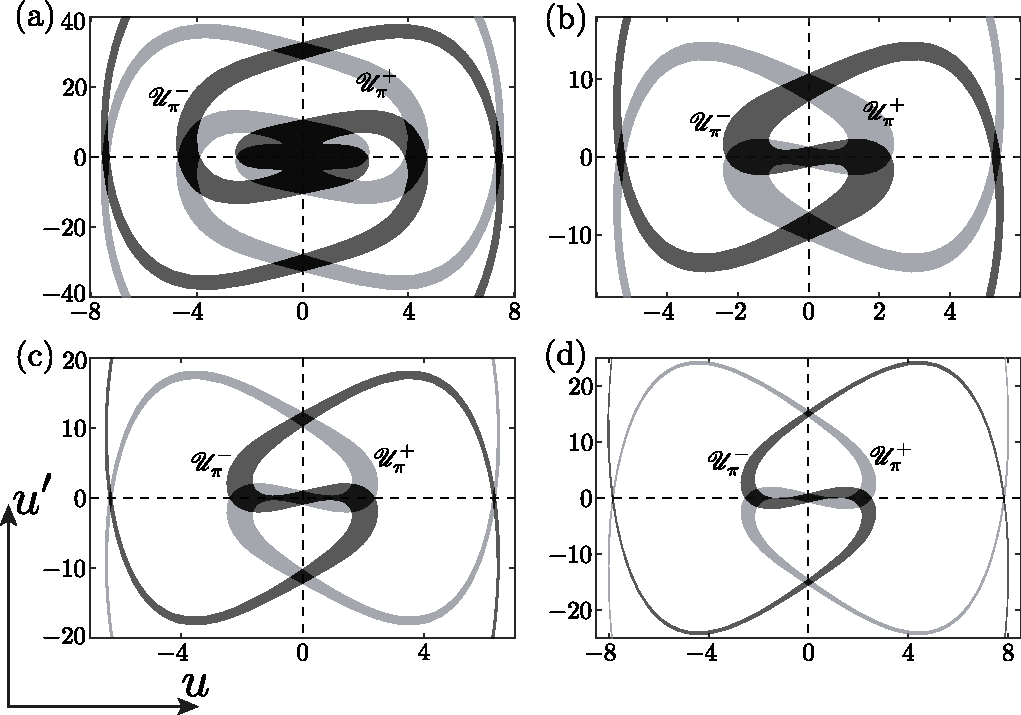
\includegraphics[scale = 1]{pic/island set emergence for cosine equation}
	\caption{
		Sets $\mathscr{U}_{\pi}^+$ (light gray), $\mathscr{U}_{\pi}^-$ (dark gray), and their intersection $\mathscr{U}_{\pi} = \mathscr{U}_{\pi}^+ \cap \mathscr{U}_{\pi}^-$ (black) for equation \eqref{eq:stationary-cosine} with different parameters $(\omega, \alpha)$.
		Panel (a): $(\omega, \alpha) = (1, 0.6)$; panel (b): $(\omega, \alpha) = (1, 0.3)$; panel (c): $(\omega, \alpha) = (1, 0.1)$; panel (d): $(\omega, \alpha) = (1, -0.1)$.
		On panels (a), (b), and (c) intersection $\mathscr{U}_{\pi}$ doesn't form an island set due to the central connected component.
		On panel (d) seven connected components of $\mathscr{U}_{\pi}$ form an island set.
	}
\label{fig:island-set-emergence-cosine}
\end{figure}

Presence of the island set structure is a first required step of our coding technique.
In Chapter~2 we established two hypotheses which must be valid, so the conditions of Theorem~\ref{thm:coding} take place.
Let's focus on the case $(\omega, \alpha) = (1.5, 0)$.
We restrict the scanning area in plane $(u, u')$ of initial conditions by seven components of $\mathscr{U}_{\pi}$.
The set $\mathscr{U}_{\pi}$ is depicted in Figure~\ref{fig:island-set-cosine}.
From that picture we conclude that Hypothesis~\ref{hypothesis:island-set} holds since each connected component of $\mathscr{U}_{\pi}$ represent a curvilinear quadrangle with monotonic boundaries, and each boundary satisfies the conditions from Definition~\ref{def:island-set}.
The connected components can be enumerated with symbols $\{D_k\}$, $k = \pm 1, \pm 2, \dots$ for the components along the $u$ axis, and $k = \pm 1\mathrm{i}, \pm 2\mathrm{i}, \dots$ for the components along the $u'$ axis.
The central component is denoted by $D_0$.
Applying this notation for the seven-component island set from Figure~\ref{fig:island-set-cosine} we have $\mathscr{U}_{\pi} = \bigcup_{k \in S_7} D_k$, $S_7 = \{ -2, -1\mathrm{i}, -1, 0, +1, +1\mathrm{i}, +2 \}$.

% TODO: Add squares and dashed lines for the island symbols.
% TODO: Consider to make this figure a little bit larger. Enlarge symbols as well.
\begin{figure}[h]
\centering
	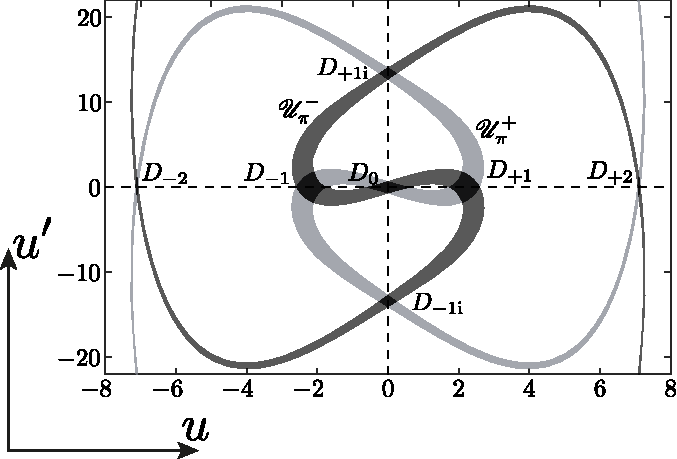
\includegraphics[scale = 1]{pic/island set to check hypotheses for cosine equation}
	\caption{
		Seven-component island set $\mathscr{U}_{\pi} = \bigcup_{k \in S_7} D_k$ (black) formed by the intersection of $\mathscr{U}_{\pi}^{\pm}$ for equation \eqref{eq:stationary-cosine} with parameters $(\omega, \alpha) = (1.5, 0)$.
	}
\label{fig:island-set-cosine}
\end{figure}

To check Hypothesis~\ref{hypothesis:strips-mapping} we use the numerical procedure described in Chapter~2 which relies on Strips Mapping Theorems from Appendix~C.
Since set $\mathscr{U}_{\pi}$ is symmetric with respect to the $u$ and $u'$ axis we can check Hypothesis~\ref{hypothesis:strips-mapping} only for four islands: $D_0$, $D_{+1}$, $D_{+2}$, and $D_{+1\mathrm{i}}$.
For each island $D_k$ we introduce a grid of values for numerical computations like we do it during the scanning procedure.
Using that grid we compute sets $H_{i, k} = \mathcal{P}(D_i) \cap D_k$ and sets $V_{k, i} = \mathcal{P}^{-1}(D_i) \cap D_k$, where $i \in S_7$.
In each point $\vb{p} \in V_{k, i}$ we construct a matrix of the 2-dimensional linear operator $D \mathcal{P}_{\vb{p}} = (a_{mn})$.
Then we analyse signs of $(a_{mn})$.
For each set $V_{k, i}$ sings of $(a_{mn})$ must have exactly one configuration specified in Theorem~\ref{thm:h-strips-mapping}.
For each island $D_k$ we also compute a numerical estimation of the lower boundary of $|a_{11}|$ values, denote it by $\mu_*$.
Corresponding histograms of $|a_{11}|$ values in logarithmic scale are presented in Figure~\ref{fig:hypotheses-validation-cosine} along with their lower boundary $\mu_*$ for each island.
Value $\mu_*$ is the numerical estimation of the value $\mu$ from Theorem~\ref{thm:h-strips-mapping}.
If the signs of values $(a_{mn})$ computed for $V_{k, i}$ sets satisfy the conditions of Theorem~\ref{thm:h-strips-mapping} and the overall estimation $\mu_* > 1$ takes place, we conclude that Hypothesis~\ref{hypothesis:strips-mapping} holds true for h-strips.

Similarly, for each set $H_{i, k}$ we construct a matrix of the linear operator $D \mathcal{P}^{-1}_{\vb{p}} = (b_{mn})$ in each point $\vb{p} \in H_{i, k}$.
We perform an estimation of the lower boundary of the values $|b_{22}|$, denote the estimated value by $\nu_*$.
If $\nu_* > 1$ and the signs of values $(b_{mn})$ computed for $H_{i, k}$ sets satisfy the conditions of Theorem~\ref{thm:v-strips-mapping}, we conclude that Hypothesis~\ref{hypothesis:strips-mapping} holds true for v-strips as well.

Complete results of our numerical analysis are presented in Figure~\ref{fig:hypotheses-validation-cosine}.
Let's provide several examples on how this picture should be treated.
Consider an island $D_{+1}$.
Operator $D \mathcal{P}_{\vb{p}} = (a_{mn})$ is computed in each point of the set $V_{+1, 0}$ and has signs configuration $\begin{psm} - & + \\ - & + \end{psm}$ on the whole $V_{+1, 0}$, i.e. $a_{11} < 0$, $a_{12} > 0$, $a_{21} < 0$, $a_{22} > 0$.
Boundaries $\alpha_{+1}^{\pm}$ of the island $D_{+1}$ are the parts of boundaries of $\mathscr{U}_{\pi}^-$ and have the form of decreasing curves, see Figure~\ref{fig:hypotheses-validation-cosine}~(b).
Boundaries $\alpha_0^{\pm}$ of the island $D_0$ are increasing curves.
It means that condition (2d) of Theorem~\ref{thm:h-strips-mapping} takes place for a pair of islands $D_{+1}$ and $D_0$.
For the sets $V_{k, i}$ all the values $|a_{11}| \ge \mu_* > 1$.
Thus, according to Theorem~\ref{thm:h-strips-mapping} we can conclude that for any h-strip $H \in D_{+1}$ its $\mathcal{P}$-image $\widetilde{H}_0 = \mathcal{P}(H) \cap D_0$ is also as h-strip and $d_{\mathrm{h}}(\widetilde{H}_0) \le (1 / \mu_*) d_\mathrm{h}(H)$.

For another example let's consider a pair of islands $D_{+1 \mathrm{i}}$ and $D_{+2}$.
Operator $D \mathcal{P}^{-1}_{\vb{p}} = (b_{mn})$ has sings configuration of the form $\begin{psm} - & - \\ + & + \end{psm}$ for all $\vb{p} \in H_{+1 \mathrm{i}, +2}$.
Boundaries $\beta_{+1 \mathrm{i}}^{\pm}$ of the island $D_{+1 \mathrm{i}}$ are decreasing curves, and boundaries $\beta_{+2}^{\pm}$ of the island $D_{+2}$ are increasing.
Estimations $\nu_* > 1$ takes place for all the sets $H_{i, k}$.
Thus, condition (1d) of Theorem~\ref{thm:v-strips-mapping} is satisfied which implies that and for any v-strip $V \in D_{+2}$ its $\mathcal{P}$-pre-image $\widetilde{V}_{+1 \mathrm{i}} = \mathcal{P}^{-1}(V) \cap D_{+1\mathrm{i}}$ is also a v-strip and $d_{\mathrm{v}}(\widetilde{V}_{+1 \mathrm{i}}) \le (1 / \nu_*) d_\mathrm{v}(V)$.
Other sets $H_{i, k}$, $V_{k, i}$ are considered in a similar way.
According to the numerical computations Theorems~\ref{thm:h-strips-mapping} and \ref{thm:v-strips-mapping} are valid for all islands $D_k$, $k \in S_7$.

% TODO: Take care of the position for this figure.
\begin{figure}[h!]
\centering
	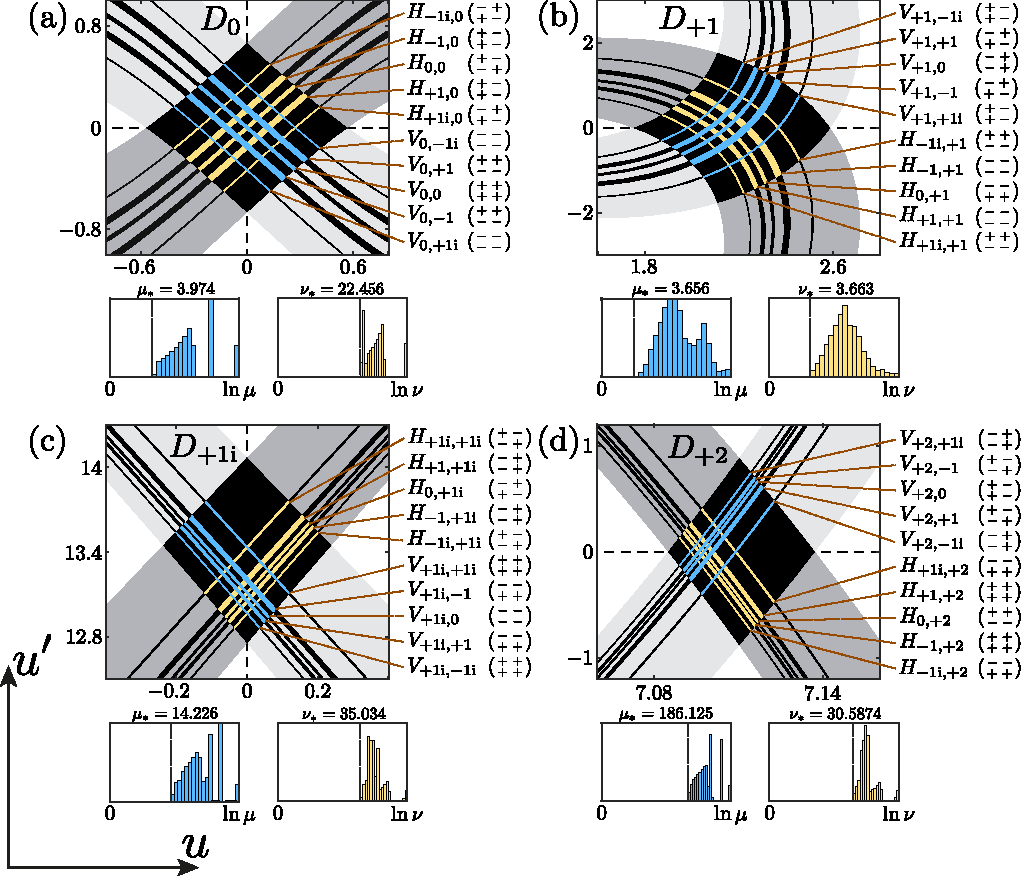
\includegraphics[scale = 1]{pic/hypotheses for cosine equation}
	\caption{
		Illustration to Hypothesis~\ref{hypothesis:strips-mapping} validation for equation \eqref{eq:stationary-cosine} with parameters $(\omega, \alpha) = (1.5, 0)$.
		Islands $D_k$ are black curvilinear quadrangles with monotonic boundaries.
		Boundaries of the set $\mathscr{U}_{\pi}^+$ (light gray) contains $\beta_k^{\pm}$ boundaries for each island $D_k$; boundaries of $\mathscr{U}_{\pi}^-$ (dark gray) contains $\alpha_k^{\pm}$ boundaries correspondingly.
		Estimations of $\mu_*$ and $\nu_*$ values are shown with histograms below each island.
		Configuration of value signs in operators $D \mathcal{P}_{\vb{p}} = (a_{mn})$, $\vb{p} \in V_{k, i}$ (blue), and $D \mathcal{P}^{-1}_{\vb{p}} = (b_{mn})$, $\vb{p} \in H_{i, k} $ (yellow) are shown from the right side of each island $D_k$.
		All of them satisfy the conditions of Theorem~\ref{thm:h-strips-mapping} (On h-strip mapping) and Theorem~\ref{thm:v-strips-mapping} (On v-strips mapping) from Appendix~C.
		Sets $H_{+2, k}$ and $V_{k, +2}$ are not depicted since they are too thin and barely visible at this scale, but all the computations have been also provided for them and the overall result satisfies the above mentioned theorems as well.
	}
\label{fig:hypotheses-validation-cosine}
\end{figure}

The procedure described above provides a numerical evidence for Hypotheses~\ref{hypothesis:island-set} and \ref{hypothesis:strips-mapping}.
That allows us to apply Coding Theorem and conclude that for Eq.~\eqref{eq:stationary-cosine} there exists a homeomorphism $\mathcal{C}: \mathcal{O}_7 \to \mathcal{S}_7$ between a subset of orbits of bounded solutions, denoted by $\mathcal{O}_7$, and a set $\mathcal{S}_7$ of bi-infinite sequences of symbols from alphabet $S_7 = \{ -2, -1\mathrm{i}, -1, 0, +1, +1\mathrm{i}, +2 \}$.
Orbits of such solutions may visit only islands $D_k$, where $k \in S_7$.
Moreover there is no any other bounded solution which orbit visits only these seven islands.
The numerical results from above can be extended to a larger island set, although it requires significant computing capacities.

Existence of the homeomorphism allows to make a conclusion on the structure of bounded solutions of Eq.~\ref{eq:stationary-cosine} 
For example Eq.~\ref{eq:stationary-cosine} admits periodic solution of period $n \pi$ for any number $n \in \mathbb{N}$.
Several periodic solutions are presented in Figure~\ref{fig:solutions-cosine}, $\pi$-periodic solution in panel (a), and $2 \pi$-periodic solutions in panels (b) and (c).
There also exists a plethora of soliton solutions.
The orbit corresponding to the soliton solution starts and ends in the central connected components; therefore, it has the code of the form $\{ \dots, 0, 0, k_1, k_2, \dots, k_N, 0, 0, \dots \}$, where symbols $k_1$ and $k_N$ are different from ``$0$''.
Some of the soliton solutions of \eqref{eq:stationary-cosine} for $(\omega, \alpha) = (1.5, 0)$ are shown in Figure~\ref{fig:solutions-cosine}, panels (d) --- (i).
The soliton solution in panel (d) is the fundamental soliton (FS) that has been already studied in \cite{SakaguchiMalomed}.
It has code $\{ \dots 0, +1, 0, \dots \}$, or $\{ \dots 0, -1, 0, \dots \}$ which is its symmetric counterpart.

Other types of localized solutions have been also found.
For example, solution, shown in panel (e), represents a so-called {\it dipole soliton} (DS) \cite{LebedevAlfimovMalomed}, which is essentially confined to a single period of pseudopotential $P(x)$.
This solution corresponds to code $\{ \dots, 0, -1\mathrm{i}, 0, \dots \}$, and its symmetric counterpart is $\{ \dots, 0, +1\mathrm{i}, 0, \dots \}$.
DS is similar to {\it sub-fundamental solitons} (SFSs) reported in \cite{MayteevarunyooMalomed, WangYanLiu, MayteevarunyooMalomedBaizakovSalerno, CuevasMalomedKevrekidisFrantzeskakis} in models with the linear lattice potential $U(x)$, as both soliton species feature the antisymmetric profile squeezed into a single cell of the underlying lattice potential (ordinary potential $U(x)$, in the case of SFS, and the pseudopotential $P(x)$, as concerns the DS).
The area of the localization of the soliton corresponding to code $\{ \dots, 0, k_1, \dots, k_N, 0, \dots \}$, where the symbols $k_1$ and $k_N$ are different from ``$0$'', is $N \pi$, i.e. it extends over $N$ periods of the underlying pseudopotential $P(x)$.
In particular, the solitons with codes $\{ \dots, 0, k, 0, \dots \}$, $k \ne 0$ (named {\it elementary solitons}), are localized, essentially, in one period of the pseudopotential. 

\begin{figure}[h]
\centering
	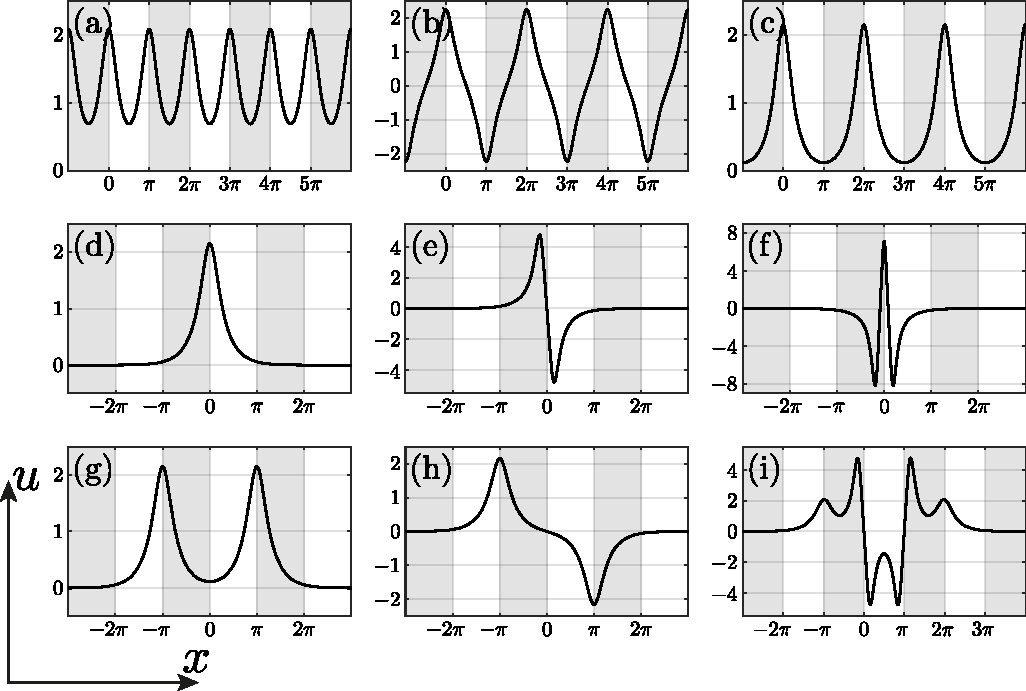
\includegraphics[scale = 1]{pic/solutions for cosine equation}
	\caption{
		Different solutions for equation \eqref{eq:stationary-cosine} with parameters $(\omega, \alpha) = (1.5, 0)$.
		Each solution has a corresponding symbolic code, this code identify the solution uniquely.
		Gray strips divide the $x$ axis according to the period $\pi$.
		First three panels represent periodic solutions, their codes have periodic structure: (a) $\pi$-periodic solution $\{ \dots, +1, +1, +1, \dots \}$; (b) $2 \pi$-periodic solution $\{ \dots, +1, -1, +1, -1, \dots \}$; (c) $2 \pi$-periodic solution $\{ \dots, +1, 0, +1, 0, \dots \}$.
		Other six panels represent localized solutions, their codes have ``$0$'' symbol to the left and right of the central block: (d) fundamental soliton with code $\{ \dots, 0, +1, 0, \dots \}$; (e) dipole soliton with code $\{ \dots, 0, -1\mathrm{i}, 0, \dots \}$ (f) elementary soliton with code $\{ \dots, 0, +2, 0, \dots \}$ (g) $\{ \dots, 0, +1, 0, +1, 0, \dots \}$ (h) $\{ \dots, 0, +1, 0, -1, 0, \dots \}$ (i) $\{ \dots, 0, +1, -1\mathrm{i}, +1\mathrm{i}, +1, \dots \}$.
	}
\label{fig:solutions-cosine}
\end{figure}

\section*{3.3 Analysis of Stability}
\addcontentsline{toc}{section}{3.3 \quad Analysis of Stability}

Stability is a critically important issue for stationary localized solutions.
By stability of localized stationary solution we mean its resistance to small perturbations.
From the perspective of real physical experiments only stable solutions can be obtained in a real experimental setup.
Here we address the stability of stationary localized solutions produced by Eq.~\eqref{eq:gpe-cosine}.
Let $u(x)$ be a solution if Eq.~\eqref{eq:stationary-cosine}.
Following the well-established approach, see e.g. \cite{JiankeYang}, let's consider small perturbations around a solution $u(x)$ of the form
\begin{equation}
	\Psi(t, x) = \left( u(x) + \widetilde{U}(t, x) \right) e^{i \omega t}; \quad |\widetilde{U}(t, x)| \ll 1,
\label{eq:perturbation}
\end{equation}
where $\widetilde{U}(t, x)$ is a complex-valued function.
Then the perturbation $\widetilde{U}(t, x)$ satisfies the linear equation
\begin{equation}
	i \widetilde{U}_t + \widetilde{U}_{xx} - \omega \widetilde{U} + (\alpha + \cos 2x) u^2 (2 \widetilde{U} + \widetilde{U}^\dagger) = 0.
\label{eq:perturbation-equation}
\end{equation}
Here dagger ``$\dagger$'' means complex conjugate.
Seeking solutions to \eqref{eq:perturbation-equation} as
\begin{equation}
	\widetilde{U}(t, x) = (v(x) + w(x)) e^{\lambda t} + (v^{\dagger}(x) - w^{\dagger}(x)) e^{\lambda^{\dagger} t}; \quad \lambda \in \mathbb{C},
\end{equation}
we arrive at the eigenvalue problem
\begin{equation}
	i
	\begin{pmatrix}
		0 & \partial_{xx} + G_1(x) \\
		\partial_{xx} + G_2(x) & 0
	\end{pmatrix}
	\begin{pmatrix}
		v \\
		w
	\end{pmatrix}
	= \lambda 
	\begin{pmatrix}
		v \\
		w
	\end{pmatrix},
\label{eq:eigenvalue-problem}
\end{equation}
where
% TODO: Consider to use $\mathcal{L}_-$ and $\mathcal{L}_+$ instead.
\begin{eqnarray*}
	&& G_1(x) = -\omega + (\alpha + \cos 2x) u^2; \\
	&& G_2(x) = -\omega + 3 (\alpha + \cos 2x) u^2.
\end{eqnarray*}

Equation \eqref{eq:eigenvalue-problem} is the linear-stability eigenvalue problem for the soliton.
Its $\lambda$-spectrum is called the linear-stability spectrum for this soliton.
The soliton is linearly stable if the spectrum produced by Eq.~\eqref{eq:eigenvalue-problem} contains at least one eigenvalue $\lambda$ with a non-zero real part, $\mathfrak{R}(\lambda) > 0$.
Otherwise, the soliton is linearly stable.
Equation \eqref{eq:eigenvalue-problem} generates spectrum consisting of continuous and discrete parts.
One can show, see e.g. \cite{JiankeYang}, that the continuous spectrum is represented by two rays, $[i\omega; +i \infty)$ and $(-i \infty; -i \omega]$, if $\omega > 0$, and by the whole imaginary axis, if $\omega < 0$.
The discrete spectrum includes zero eigenvalue $\lambda = 0$.
It is easy to see that other eigenvalues of discrete spectrum of Eq.~\eqref{eq:eigenvalue-problem} have the following symmetry properties: if $\lambda$ is an eigenvalue, then so are $\lambda^{\dagger}$, $-\lambda$, and $-\lambda^{\dagger}$.
This means that these eigenvalues always appear in pairs or quadruples.

\subsection*{3.3.1 Fourier Collocation Method}

To find discrete eigenvalues numerically we use so-called Fourier Collocation Method (FCM) described in \cite{JiankeYang}.
This method is very efficient to find {\it exponential instabilities} that appear due to real eigenvalues.
We also say that solution {\it oscillatory unstable} if the spectrum has quartets of complex with non-zero real parts.

To apply FCM, we first truncate the infinite $x$-axis into a finite interval into  a finite interval $[-L/2; L/2]$, where $L$ is the length of the interval.
Length of the interval is considered to be large enough to cover soliton solution localization well.
On this interval we expand the eigenfunctions $[v(x); w(x)]^T$ and functions $G_1$, $G_2$ into Fourier series:
\begin{eqnarray}
	&& 	v(x) = \sum \limits_n a_n e^{i n k_0 x}; \quad w(x) = \sum \limits_n b_n e^{i n k_0 x}, \label{eq:eigenfunctions-expansion} \\
	&& G_1 = \sum \limits_n c_n^{(1)} e^{i n k_0 x}; \quad G_2 = \sum \limits_n c_n^{(2)} e^{i n k_0 x} \label{eq:g-functions-expansion},
\end{eqnarray}
where $k_0 = 2 \pi / L$.
After substitution of \eqref{eq:eigenfunctions-expansion} and \eqref{eq:g-functions-expansion} into \eqref{eq:eigenvalue-problem}, we have the following eigenvalue system fro the coefficients $a_j$, $b_j$:
\begin{eqnarray}
	&& -(k_0 j)^2 b_j + \sum \limits_n 	c_n^{(1)} b_{j - n} = -i \lambda a_j; \\
	&& -(k_0 j)^2 a_j + \sum \limits_n 	c_n^{(2)} a_{j - n} = -i \lambda b_j,
\end{eqnarray}
where $-\infty < j < +\infty$.
Truncating the number of Fourier modes to $-N \le j \le N$, this infinite-dimensional eigenvalue problem can be reduced to the finite-dimensional one:
\begin{equation}
	i
	\begin{pmatrix}
		0 & D + C_1 \\ D + C_2 & 0
	\end{pmatrix}
	\begin{pmatrix}
		A \\ B
	\end{pmatrix}
	= \lambda
	\begin{pmatrix}
		A \\ B
	\end{pmatrix},
\label{eq:eigenvalue-problem-matrix}
\end{equation}
where
\begin{eqnarray*}
	&& D = (ik_0)^2 \mathrm{diag}(-N, -N+1, \dots, N-1, N)^2; \\
	&& A = (a_{-N}, a_{-N+1}, \dots, a_N)^T; \quad B = (b_{-N}, b_{-N+1}, \dots, b_N)^T,
\end{eqnarray*}
and matrices $C_1$, $C_2$ are of the form of Toeplitz matrices
\begin{equation}
	C_{1,2} =
	\begin{pmatrix}
		c_0^{(1,2)} & c_{-1}^{(1,2)} & \cdots & c_{-N}^{(1,2)} & 0 & \cdots & 0 \\
		c_1^{(1,2)} & c_0^{(1,2)} & c_{-1}^{(1,2)} & \ \ddots & \ddots & \ddots & \vdots \\
		\vdots & c_1^{(1,2)} & c_0^{(1,2)} & c_{-1}^{(1,2)} & \ddots & \ddots & 0 \\
		c_N^{(1,2)} & \ddots & \ddots & \ddots & \ddots & \ddots & c_{-N}^{(1,2)} \\
		0 & c_N^{(1,2)} & \ddots & \ddots & \ddots & \ddots & \vdots \\
		\vdots & \ddots & \ddots & \ddots & \ddots & \ddots & \vdots \\
		0 & \cdots & 0 & c_N^{(1,2)} & \cdots & c_1^{(1,2)} & c_0^{(1,2)}
	\end{pmatrix}.
\end{equation}
The matrix eigenvalue problem \eqref{eq:eigenvalue-problem-matrix} can be solved by any matrix eigenvalue problem solver.
Solution of the eigenvalue problem gives $2N + 1$ eigenvalues.
In our computations we used $N = 256$ and $N = 512$ and got nearly identical spectrums.
From the practical point of view for the linear-stability analysis the number of Fourier modes can be relatively small, since eigenvalues for the higher modes have zero real part.

\subsection*{3.3.2 Evolutionary Simulation}

To control linear-stability analysis and get additional confidence in stability of localized solutions we also performed a numerical simulation of their evolution.
For that purpose Trofimov-Peskov finite-difference scheme \cite{TrofimovPeskov} for numerical solution of the Gross-Pitaevskii \eqref{eq:gpe} equation was used. 
The scheme preserves several invariants of the problem: the norm of the solution
\begin{equation}
	N = \int \limits_{-\infty}^{+\infty} |u(x)|^2 dx,
\label{eq:norm}
\end{equation}
and its energy
\begin{equation}
	E = \int \limits_{-\infty}^{+\infty} \left( |u'(x)|^2 + U(x) |u(x)| - \dfrac{1}{2} P(x) |u(x)|^4 \right) dx.
\label{eq:energy}
\end{equation}
The scheme is implicit, its realization implying iterations for the calculation of values in each temporal layer, but it allows running computation with larger temporal step.
In order to reveal instability (if it is), the soliton profile was perturbed at the initial moment with a small perturbation.
A finite spatial domain $[-5 \pi; 5 \pi]$ was used, with reflection of radiation from boundaries eliminated by means of absorbing boundary conditions.
During our analysis we got consistent results between the linear stability and evolutionary simulation.

\subsection*{3.3.3 Results of Linear Stability Analysis}

With the help of FCM, a great number of localized stationary solutions of equation \eqref{eq:gpe-cosine}, represented by different codes, were analyzed.
Due to the infinite number of essentially different solitons, it's not possible to preform a comprehensive stability analysis of all localized solutions.
However, we observed that a majority of the solitons are linearly unstable, thus being physically irrelevant solutions.
{\it Stable solitons} can be categorized as follows:
\begin{itemize}
	\item[(a)] among the elementary solitons, it was found that FS and DS are {\it linearly stable}, under some restrictions on parameters $\omega$ and $\alpha$, while other elementary solitons were found to be unstable;
	\item[(b)] there are stable localized solutions of the form of FS complexes --- for instance, with codes $\{ \dots, 0, +1, -1, +1, 0, \dots \}$ and $\{ \dots, +1, 0, -1, 0, \dots \}$.
\end{itemize}

\begin{figure}[h!]
\centering
	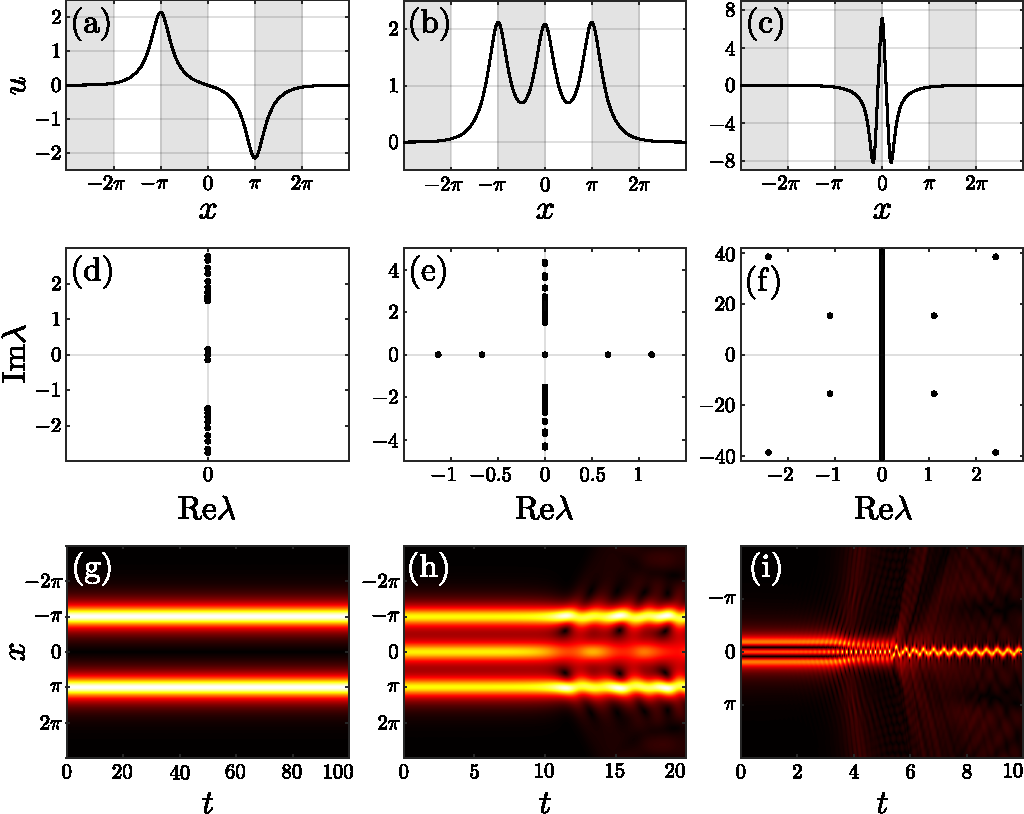
\includegraphics[scale = 1]{pic/stability demonstration for cosine equation}
	\caption{
		Examples of stability analysis for localized solutions of equation \eqref{eq:gpe-cosine} with parameters $(\omega, \alpha) = (1.5, 0)$.
		First three panels represent profiles of solutions of different codes: (a) $\{ \dots, 0, +1, 0, -1, 0, \dots \}$; (b) $\{ \dots, 0, +1, +1, +1, 0, \dots \}$; (c) $\{ \dots, 0, +2, 0, \dots \}$.
		Panels (d), (e), and (f) are the corresponding $\lambda$-spectrums for the solutions above.
		According to them, solution in panel (a) is linearly stable.
		Solution in panel (b) is exponentially unstable, while solution in panel (c) is oscillatory unstable.
		Linear-stability analysis match the results of evolutionary simulation presented in panel (g), (h), and (i).
	}
\label{fig:stability-cosine}
\end{figure}

Several localized solution, their linear-stability spectrums, and corresponding results of evolutionary simulation are in Figure~\ref{fig:stability-cosine}.
Panel (a) corresponds to a stable localized solution of code $\{ \dots, 0, +1, 0, -1, 0, \dots \}$.
Such solution can be considered as a combination of two FSs of codes $\{ \dots, 0, +1, 0, \dots \}$ and $\{ \dots, 0, -1, 0, \dots \}$.
Another similar combination of code $\{ \dots, 0, +1, +1, +1, 0, \dots \}$ in panel (b) is unstable.
Elementary soliton of code $\{ \dots, 0, +2, 0, \dots \}$ from panel (c) is unstable as well as any other elementary solitons except of FS and DS.
Other examples can be found in our work \cite{LebedevAlfimovMalomed}.

Combination of coding technique and linear-stability analysis together give a powerful tool of visualization of stationary localized solutions stability for equation of type \eqref{eq:gpe} with periodic potential and pseudopotential.
If it's possible to find such parameters that the Theorem~\ref{thm:coding} is applicable, then for these parameters we can apply coding and describe at least a huge subset of bounded solutions.
After that one can vary one of the parameters using a numerical grid and perform a numerical continuation for the described solutions to the non-coding area of parameters.
During the numerical continuation of solutions we can compute linear-stability spectrums in each point of the parameters grid.
Then we can parametrized the obtained solutions, for example using their norm \eqref{eq:norm}, plot the branches of different solution families and color the stability regions.

Illustration of the described idea for Eq.~\eqref{eq:gpe-cosine} is presented in Figure~\ref{fig:branches-with-stability}.
In that figure several branches of solutions are depicted in $(N, \omega)$ axes, while parameter $\alpha = 0$.
Regions of linear stability are marked with bold black lines.
One can see that FS solution of code $\{ \dots, 0, \pm 1, 0, \dots \}$, branch (I), and solution of code $\{ \dots, 0, \pm 1, 0 \mp 1, 0, \dots \}$, branch (II), are mostly stable and loose their stability near the point $\omega = 0$.
Dipole soliton, branch (IV), exists for $\omega > \omega^*$ and has an $\omega$-region of stability.
At $\omega^* \approx 0.265$, the DS family, coded by $\{ \dots, 0, \pm 1\mathrm{i}, 0, \dots \}$, undergoes a saddle-node bifurcation and annihilate with the family coded by $\{ \dots, 0, \mp 1, \pm 1\mathrm{i}, \pm 1, 0, \dots \}$.

% TODO: Consider to move solution panels lower.
\begin{figure}[h]
\centering
	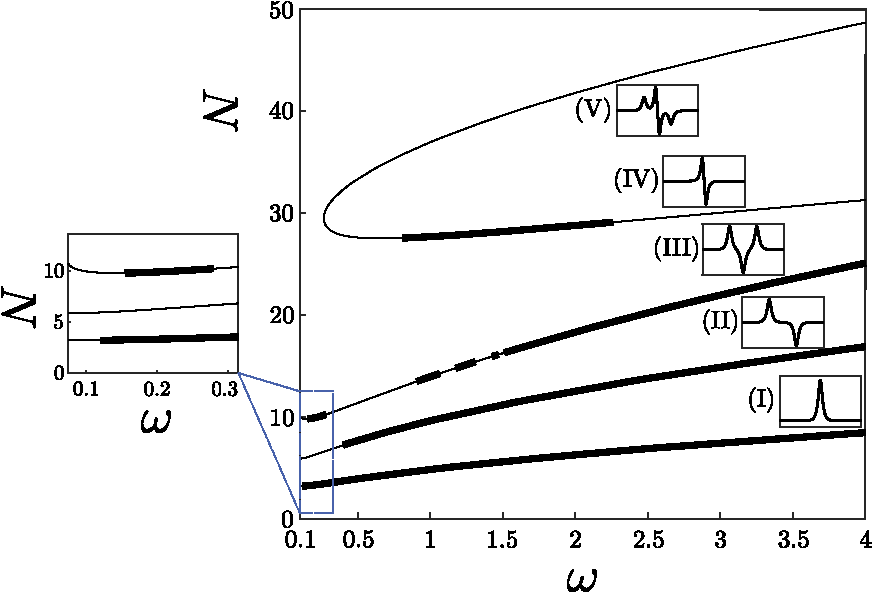
\includegraphics[scale = 1]{pic/branches for cosine equation}
	\caption{
		Branches of solutions for Eq.~\eqref{eq:gpe-cosine} and their linear stability.
		Branch (I) represent fundamental soliton family of code $\{ \dots, 0, \pm 1, 0, \dots \}$.
		Branches (II) and (III) are FS complexes of codes $\{ \dots, \pm 1, 0, \mp 1, 0, \dots \}$ and $\{ \dots, \pm 1, \mp 1, \pm 1, 0, \dots \}$ correspondingly.
		Dipole soliton family of code $\{ \dots, 0, \pm 1\mathrm{i}, 0, \dots \}$ is presented by the branch (IV).
		It coalesces at $\omega = \omega^*$ with family $\{ \dots, 0, \mp 1, \pm 1\mathrm{i}, \pm 1, 0, \dots \}$ of branch (V).
		Linear stability regions are colored with bold black lines.
	}
\label{fig:branches-with-stability}
\end{figure}

\subsubsection*{3.3.4 Stable Dipole Soliton}

As an outcome of our analysis for physical applications, the most significant finding is the existence of stable DS family, which was not previously considered in the setting of GPE with periodic pseudopotential.
Existence of such family is also predicted by variational approximation method, see \cite{LebedevAlfimovMalomed}.
The DS family may be parametrized by $\omega$.
The norm of the DS grows with the growth of $\omega$.
Although the DS is very similar, in its shape, to the sub-fundamental solitons in systems with periodic potential, the DS in the present model is not sub-fundamental, as its norm os {\it higher} than that of the FS existing for the same $\omega$, see Figure~\ref{fig:branches-with-stability}.
Evolutionary simulation showed that if for some $\omega$ the DS is unstable, then it transforms into the FS after some time.
An example of that is provided in Figure~\ref{fig:stability-dipole-soliton}.

\begin{figure}[h]
\centering
	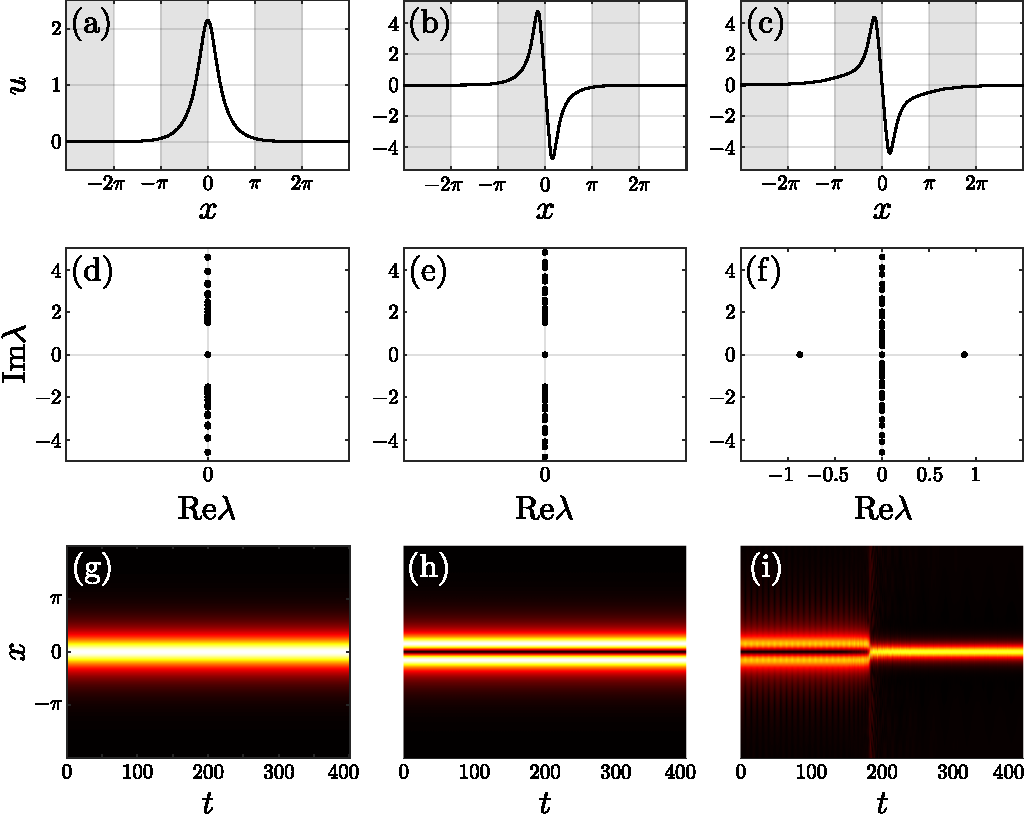
\includegraphics[scale = 1]{pic/dipole soliton stability}
	\caption{
		Stability of dipole soliton.
		Panel (a) represent a stable fundamental soliton (FS) for parameters $(\omega, \alpha) = (1.5, 0)$.
		Panel (b) corresponds to stable dipole soliton (DS) for $(\omega, \alpha) = (1.5, 0)$.
		Unstable DS is presented in panel (c) for parameters $(\omega, \alpha) = (0.4, 0)$.
		It's exponentially unstable and  during our simulation at $t \approx 200$ transforms into a stable fundamental soliton.
	}
\label{fig:stability-dipole-soliton}
\end{figure}

\section*{3.4 Summary}
\addcontentsline{toc}{section}{3.4 \quad Summary}

In this chapter we studied stationary solutions of Gross--Pitaevskii equation \eqref{eq:gpe} with presence of periodic pseudopotential $P(x)$ of the cosine form \eqref{eq:cosine-pseudopotential}, while potential $U(x)$ is absent.
We focused on localized solutions as they are of particular interest for physical experiments.
Periodicity of pseudopotential $P(x)$ allowed us to apply coding technique from Chapter~2. % \ref{chapter:II}
We provided a numerical evidence for Hypotheses~\ref{hypothesis:island-set} and \ref{hypothesis:strips-mapping}, which allow to apply Theorem~\ref{thm:coding}, and concluded that there exist a homeomorphism between a subset of bounded solutions and bi-infinite symbolic sequences from some alphabet.
Existence of the homeomorphism reveal the complex nature of stationary solutions. 
Like we saw it in Chapter~2 presence of periodic pseudopotential that alters its sign along the period generates a great variety of different stationary solutions.
We apply linear-stability analysis to identify physically relevant localized solutions among them.
Outcome of our analysis is the existence of stable dipole soliton (DS) family previously not considered in this setting.
Results of our finding were published in \cite{LebedevAlfimovMalomed}.
